\newpage
\appendix
    \addtocontents{toc}{\protect\setcounter{tocdepth}{1}}
    \renewcommand\thefigure{\thesection.\arabic{figure}} %Number figure A1, A2, etc.
    \renewcommand{\thetable}{A.\arabic{table}} %Number tables A1, A2, etc.
    \setcounter{figure}{0} %Start numbering from 1   
    \setcounter{table}{0}


\section{Appendices}
    \subsection{Original Thesis Challenge}\label{app_sec_challenge}
        \epigraph{''Desarrollar una metodología para analizar la conversación chilena en twitter sobre un tópico específico, considerando afiliación política de los usuarios. Describir las narrativas asociadas que aparecen a lo largo del tiempo y la estructura de red de los grupos involucrados. Aplicar la metodología desarrollada utilizando como tema de prueba inmigración.''}{--- Claudio Villegas Oliva, Chilean Communication Office}
    
    
    
    
    \subsection{Applying the Methodology}\label{app_sec_meth}

            This section presents how we have applied the general methodology presented in Section \ref{sec_meth_gene}.
            
            All the notebooks can be found in the \texttt{methodology\_immigration}-folder of the GitHub repository (particularly in the subfolder \texttt{new\_topic}).
   
        %\paragraph{Step 1: \texttt{twarc2}-Query1 Semantic Link}
        \paragraph{Step 1} 
            We input the term ''immigration'' into {\it Semantic Link}. Utilizing our domain knowledge, we exclude words returned by {\it Semantic Link} that $(i)$ are unrelated with immigration in Chile such as ''Aliyah'' or $(ii)$ highly related to other topics such as ''unskilled''. We translate the relevant words and then we run the notebook\footnote{The words that we used were: inmigración  migración, migrante,migrantes, inmigrante, inmigrantes, emigrantes, deportación, deportado, deportados, refugiado and refugiados} \texttt{1.1\_First\_Query\_to\_Twarc.ipynb} with our specified list of semantically linked keywords to return the first corpus with geolocated tweets from Chile. See Appendix \ref{appsec_twarc_query1} for our full query for Step 1.
    
        %To obtain the first corpus of tweets, we follow the step described previously.
        %To find our first set of words, we searched in the Semantic Link webpage our main topic (immigration) and manually selected the words that are most relevant and  related with our topic. For instance, we exclude the word Aliyah because it is irrelevant in our case, or we exclude the word unskilled because it is related with many other topics. 
        %Using the API, we download tweets specifying the set of words, the location and the period we are interested in studying. (See Appendix \ref{appsec_twarc_query1} for full query)
        
            \newline\indent
        \textbf{Output}: Corpus of geolocated tweets from Chile that contain semantically linked keywords to the term ''immigration''. The resulting corpus from Step 1 had 15,339
        
        \paragraph{Validation:} Defining the appropriate set of words is of great importance. Including a too narrow list in the tweet retrieve search, would potentially fail to capture relevant tweets. Specifying a too broad list, would potentially capture too much noise and risks exceeding the maximum download limits set by the API. In this step we try different sets of words and we explored the outputs.
    
    
        %\paragraph{Step 2: \texttt{twarc2}-Query2 Semantic Link + Country Contextual} 
        \paragraph{Step 2} 
        We extend the first list of semantically linked keywords to ''immigration'' by exploring the output retrieved from Step 1. We investigate the top 200 words and hashtags, and from this select the terms ''venezolanos'', ''haitianos'',''xenofobia'' and ''extranjeros'' to add to our list of keywords. Further, we again utilize our domain knowledge and also we created a list of Chilean related words with the last name of the president and the two candidates in last election, names of cities, and all the regional capitals, most common slangs and the account of Chilean Government to obtain tweets related with Chile. The first query require that the tweets have to contain one immigration related word and one Chilean related word. The second one require one immigration related word and a tweet geo-located in Chile. We run the notebook \texttt{1.2\_Adding\_words\_looking\_the\_Chilean\_context} to download the corresponding tweets. See Appendix \ref{appsec_twarc_query2} for our full query for Step 2.
        
        %To extend the first list of words, we explore the output retrieved as described previously (200 top words and hashtags). In our case, we added the words “venezolanos”, “haitianos” in this step.
        %To restrict by location, we use manual input and our field knowledge as well as the API's option. The additional words specified include the last name of the president and the two candidates in last election, names of cities, and all the regional capitals. Then, using this final list of keywords, we downloaded the corresponding tweets. See Appendix \ref{appsec_twarc_query2} for our full query for Step 1.
        
            \newline\indent
        \textbf{Output}: Corpus of geolocated tweets from Chile or tweets that used Chilean related words that contain semantically or contextual linked keywords to the term ''immigration''. The resulting corpus from Step 2 had 502,510 tweets.
        
        %Corpus with tweets that contain immigration related words (by semantic link and Chilean Twitter context), restricted by location using Chilean location related words (personal domain knowledge) or geo-located in Chile (API option). 
        
        
        \paragraph{Step 3}
    
        To filter the corpus from Step 2 by citizens that are either located in Chile or Chileans living abroad apply the criteria outlined in Step 3 in Section \ref{sec_meth_gene} as follows. We only include Twitter users that have one or more of the following in their self-written author descriptions and/or locations: $(i)$ A Chilean flag as an emoji (''\texttt{flag:chile}''); $(ii)$ {\it 'chile'} as a regular expression, including derivations thereof, such as {\it 'chileno'}, {\it 'chilena'}; $(iii)$ An unambiguous Chilean city either as an $n$-gram or unigram. We run the notebook \texttt{1.3\_Filter\_by\_Chileans} to filter the Twitter users. See Appendix Table \ref{app:tab_unis} for the list of unigram excluded (ambiguous) list of cities in Chile and the included ones; Appendix Table \ref{app:tab_ngrams} presents the list of $n$-gram excluded (ambiguous) list of Chilean cities and the included ones.
        
        
        %Since the previous corpus still included tweets from non-Chileans. We aim to address this issue using our location filtering methodology and directly extracting information from Twitter users. We only include authors whose self-written location and/or biographies include :
    
        %\begin{enumerate}
        %    \item 
        %    A Chilean flag as an emoji
            
        %    \item
        %    {\it 'chile'} as a regular expression -- including derivations thereof, such as {\it 'chileno'}, {\it 'chilena'}, etc.
            
        %    \item
        %    An unambiguous Chilean city either as an $n$-gram or unigram.\footnote{By 'unambiguous' we refer to a city name which is not also a city or country name in another country than Chile (so e.g. not {\it 'Florida'}, {\it 'El Salvador'}, {\it 'Cartagena'}, {\it 'San Carlos'}, {\it 'Los Lagos'}, etc.).} The list of Chilean cities is obtained from Wikipedia.   
                        
        %\end{enumerate}
        
        
        \textbf{Output}: List of authors located in Chile or Chilean citizens tweeting about immigration as specified by the semantically linked keywords to the term ''immigration'' and immigration-Chile-contextual keywords. The output from this step was a list of 45,550 unique authors.
    
        
        \textbf{Validation}: Reviewing the list of Twitter users obtained after Step 3, we are confident that the vast majority of tweets in the resulting corpus are written by Twitter users located in Chile or Chilean citizens by reviewing a random subsample of authors' location and description, the top 20 author locations, and wordcloud of author description. See Appendix Table \ref{random_loc_desc}, Appendix Figure \ref{appfig_top20_auth_locs} and Appendix Figure \ref{appfig_auth_desc_cloud} for the previously mentioned investigations, respectively.\footnote{Appendix Figure \ref{appfig_top20_auth_locs} shows that in the 20 most popular author locations in our sample are all from Chile. Appendix Figure \ref{appfig_auth_desc_cloud} shows the wordcloud of author biographies where domain knowledge confirms is that the words to a large degree are regarding Chilean users. The wordcloud includes Chilean words and phrases related to the topic of immigration in the country.}
        
        
        \paragraph{Step 4} 
        
        This step retrieves all the tweets about immigration from Chilean authors identified in Step 3. We add the the list of semantic linked and Chile-contextual keywords from Step 2 into the \texttt{twarc2} query. We also again specify the time frame. We run the notebook \texttt{1.4\_Download\_all\_related\_tweets\_from\_local\_authors} to obtain the full list of tweets from the specified authors.\footnote{This is a computationally intensive task. The list of authors was split into three and ran on separate computers. Each query took between 5-7 hours to complete in each of the machines.}
        %(It is not needed to filter again by location given the Step 3.)
        See Appendix \ref{appsec_twarc_query4} for our full query for Step 4.\footnote{Considering that twarc has a maximum number of characters for a single query, we split the authors list and we create a list of queries that we run from a txt file using the option searches.}
        
        \newline\noindent
        
        \textbf{Output}: Corpus with tweets that contain-immigration related words (by semantic link and Chilean Twitter context), 
        only included Twitter users that are either located in Chile or Chilean citizens, and are active in the conversations on immigration. The resulting corpus from Step 4 had 574,219 tweets.
        
        \paragraph{Validation}
            
            To ensure that our methodology works as intended up to Step 4, we analyze a random selection of Twitter users in the corpus and investigated their author description and location. We have also looked at the most common author location and word clouds of the author descriptions. This is done for our specific application on the topic of immigration in Chile and is presented in
            Appendix Figures \ref{appfig_top20_auth_locs} and \ref{appfig_auth_desc_cloud}. This exploratory analysis gives us confidence that the methodology works as intended and that the vast majority of tweets in the resulting corpus are written by Twitter users from the country studied. However, the corpus after Step 4 can still contain noise and tweets that do not solely pertain to the topic of interest.
        
                                
        \paragraph{Step 5} 
        
        The corpus returned from Step 4 still contains some irrelevant tweets. We check this by looking at the top words, hashtags, etc. E.g. we find a multitude of tweets regarding football matches between the Chilean and Venezuelan national football teams. Using the word- and hashtag-based filtering approach as described in Step 5 in Section \ref{sec_meth_gene}, we clean our corpus from irrelevant tweets.\footnote{We exclude the tweets that contain the hashtags: 'apostilla','25deJulio','venezolanosenelmundo','vamoscolocolo','vamoslau' and the tweets that contain the words:'gol','futbol','foul','apostilla','futbolista'} The total number of tweets that we\ remove in Step 5 is 218.
        
        \newline\noindent
        
        \textbf{Output}: Corpus from Step 4 with noise filtered out. This output is our final data set to analyze and had 573,999 tweets from 45,525 unique authors.
        
         \paragraph{Validation}
        We reviewed a random sample of 200 tweets after this step to ensure that mainly of our corpus contain tweets related to immigration in Chile. 187 of these tweets are related to our topic of interest.
        
        
        
        \paragraph{Step 6} 
        
         Here aim to characterize the authors by their political affiliation. To do so, we label the users according to the candidate that they supported in the last election. (this can be done also by ML models, but it can increase the uncertainty of measurements)
        
        Our first step was to take a list of left and right politicians and download their tweets during the electoral period. From this data set, we extract the 15 most popular hashtags for each affiliation, previous a manually filtering according with hashtags that specifically support one of the candidates. Table \ref{tab_hashtag_left_right_split} shows the specific hashtags chosen to label Twitter users in the corpus into left- and right-leaning political affiliation, respectively.
        
        
        
        %\subsubsection{Exploring the Final Corpus with Tweets about Immigration in Chile}\label{sec_res_corp}
    
        %\textcolor{red}{Figure \bf ???} shows a random selection of ten tweets from the corpus.
        
        \begin{table}[!htb]
            %\footnotesize
            \centering
            \subfile{tabs/hashtag_left_right_split}
            
            \caption{Hashtags to Label Twitter Users from Corpus into Left- And Right-Leaning Political Affiliation}
            
            \floatfoot{\it 
            Notes:  Textual preprocessing steps include lowercase enforcement and converting Spanish special characters (e.g. á, ñ, etc.) into corresponding non-accentuated ones.
            \\
            Data Source: Retrieved from Twitter API utilizing the \texttt{twarc2} command line tool, spanning the time frame Oct 19\textsuperscript{st} 2021 -- Dec 20\textsuperscript{th}, 2021 (electoral period).}
            \label{tab_hashtag_left_right_split}
        \end{table}
        
        \textbf{Output}: List of right leaning hashtags and left leaning hashtags.
    
    
        \paragraph{Step 7} 
        
        Using the previous list of hashtags we download all the tweets from the users that have tweets in the output of the step 5 in the electoral period that used one of the political hashtags. We labeled as left leaning all the authors that used more than 40 left hashtags during the campaign and that more than 80\% of the political hashtags that they used are from the list of left leaning hashtags. We do the same for the right leaning.
        
        \textbf{Output}: A list of users that tweet about immigration with their political affiliation. The dimensions of the data frame with authors labeled left or right was 9,606 (21\% of all our authors). We merge this information in our previous data set, to obtain labeled tweets and we add the label "Unlabeled" to all the users that didn't have Right or Left label. 
        
        \textbf{Validation}: Reviewing of a random sample of 40 tweets for each affiliation during the electoral period (the tweets that we used to label users), we found that 40/40 tweets from right wing users supports one of the right wing candidates, and 39/40 tweets from left wing users support one of the left wing candidates, only 1/40 was neutral.
        
        
        \paragraph{Step 8} 
        
        With the same list of keywords that we have from step 2, we download from twarc all the retweets from our list of users that contains one of the keywords. After with the plugin networks, we obtain a \texttt{.csv}-file with the necessary information to create the network (who retweeted, who received the retweet and the amount of retweets that the second users gives to the first one). Adding the previous information about labels, we create the network considering only the retweets between two users that we have in our previous list. Each node has an attribute with their political affiliation and each edge has a weight indicating the number of retweets. 
        
        \textbf{Output}: Network of retweets with Chilean users that talk about immigration during the period of interest. The network has 45,525 nodes (users) and 578,383 edges (retweets between users).

    
        
       
        
        
    \subsection{Full \texttt{twarc2} Queries for Application of Methodology}\label{appsec_twarc_queries}
    
    \subsubsection{Full \texttt{twarc2} Query for Step 1}\label{appsec_twarc_query1}
        \begin{verbatim}
twarc2 search --archive "(inmigración OR inmigracion OR migración OR migracion OR migrante 
OR migrantes OR inmigrante OR inmigrantes OR emigrantes OR deportación OR deportacion OR deportado 
OR deportados OR refugiado OR refugiados) place_country:CL -is:retweet" --start-time "2020-11-01" 
--end-time "2022-04-11"   
        \end{verbatim}
        
    \subsubsection{Full \texttt{twarc2} Queries for Step 2}\label{appsec_twarc_query2}
        \begin{verbatim}
twarc2 search --archive "(inmigracion OR  migracion OR migrante OR migrantes OR inmigrante 
OR inmigrantes OR emigrantes OR deportacion OR deportado OR deportados OR refugiado OR refugiados 
OR venezolanos OR extranjeros OR xenofobia OR haitianos) place_country:CL -is:retweet" 
--start-time "2020-11-01" --end-time "2022-04-11" 

twarc2 search --archive "(inmigracion OR  migracion OR migrante OR migrantes OR inmigrante 
OR inmigrantes OR emigrantes OR deportacion OR deportado OR deportados OR refugiado OR refugiados 
OR venezolanos OR extranjeros OR xenofobia OR haitianos) (chile OR santiago OR iquique OR arica 
OR piñera OR pinera OR boric OR kast OR valparaiso OR antofagasta OR colchane OR copiapo OR 
coquimbo OR rancagua OR talca OR conce OR temuco OR puerto montt OR valdivia OR coyhaique OR 
punta arenas OR weon OR weona OR sebastianpinera OR gabrielboric OR joseantoniokast OR 
GobiernodeChile) -is:retweet" --start-time "2020-11-01" --end-time "2022-04-11"
        \end{verbatim}
        
    \subsubsection{Full \texttt{twarc2} Query for Step 4}\label{appsec_twarc_query4}
        \begin{verbatim}
twarc2 search --archive "(inmigracion OR  migracion OR migrante OR migrantes OR inmigrante OR 
inmigrantes OR emigrantes OR deportacion OR deportado OR deportados OR refugiado OR refugiados 
OR venezolanos OR extranjeros OR xenofobia OR haitianos)(from:user1 OR from:user2 OR ...) 
-is:retweet" --start-time "2020-11-01" --end-time "2022-04-11"
        \end{verbatim}
        

        
    \subsubsection{Full \texttt{twarc2} Query for Step 6}\label{appsec_twarc_query6}
        \begin{verbatim}

twarc2 timelines --use-search --start-time "2021-10-19" --end-time "2021-12-20" left_accounts.txt

twarc2 timelines --use-search --start-time "2021-10-19" --end-time "2021-12-20" right_accounts.txt   
        \end{verbatim}
        
 
      \subsubsection{Full \texttt{twarc2} Query for Step 7}\label{appsec_twarc_query7}
        \begin{verbatim}
twarc2 search "(#boricpresidente OR #seguimos OR #boricpresidentedechile OR #apruebodignidad OR 
#rutaesperanzaxboric OR #boricnosune OR #boricpresidente2022 OR #unmillondepuertasxboric OR 
#1millondepuertasxboric OR #meunoconboric OR #ahorayasna OR #boricpresidentedechile2022 OR 
#boricenprimeravuelta OR #vota1 OR #paravivirmejor OR #atreveteconkast OR #kastpresidente2022 OR 
#kastpresidente OR #vota2votakast OR #atreveteporchile OR #sepuede OR #todochileconkast OR 
#atreveteconkast OR #kastledaesperanzaachile OR #chilevotakast OR #atrevidos OR #consichelsepuede 
OR #sichelpresidente OR #atrevidosporkast OR #votakast OR #mujeresporkast)
(from:user1 OR from:user2 OR from:user3..."--start-time "2021-10-19" --end-time "2021-12-20"
        \end{verbatim}
        
         \subsubsection{Full \texttt{twarc2} Queries for Step 8}\label{appsec_twarc_query8}
        \begin{verbatim}
twarc2 search --archive "(inmigracion OR  migracion OR migrante OR migrantes OR inmigrante 
OR inmigrantes OR emigrantes OR deportacion OR deportado OR deportados OR refugiado OR refugiados 
OR venezolanos OR extranjeros OR xenofobia OR haitianos)(from:user1 OR from:user2 OR ...) 
is:retweet" --start-time "2020-11-01" --end-time "2022-04-11" output_file.json

twarc2 network output_file.json --format csv network_final.csv --edges retweet


        \end{verbatim}  
   
    
    \subsection{Theory for Network Analysis}\label{appsec_theory}\label{appsec_theory_net}
    Our project mainly presents simple descriptive measures such as counts, percentages, etc. which we assume readers to already be familiar with. However, some more advanced measures are used, especially in our networks analysis part, and this section provides the mathematical definitions of these measures. %Non-technical readers can skip this section.

    %\subsubsection{Text Analysis Measures}\label{appsec_theory_txt}
        
        %\paragraph{$TFIDF$-Weighting}
            %Term frequency–inverse document frequency is a way of downweighting frequent terms and upweighting less frequent ones. The term frequency ($TF$) part for term $i$ for user $j$ is
            %\begin{align}
             %   TF_{ij} = \frac{n_{ij}}{\sum_k n_{k,j}}
            %\end{align}
            %where $n_{ij}$ is the number of times term $i$ occurs in all tweets produced by user $j$, and $\sum_k n_{k,j}$ is the total number of terms in all tweets produced by user $j$. 
            
             %   \newline \indent
            %The inverse document frequency ($IDF$) part for term $i$ is defined as
            %\begin{align}
            %    IDF_i = \log \frac{\lvert U \rvert}{\lvert U_i \rvert }
            %\end{align}
            %where $U$ is the set of all users, and $U_i$ is the subset of users who produced term $i$.
        
            %    \newline \indent
            %Finally, the complete the $TFIDF$-weight for term $i$ by user $j$ is calculated as follows
            %\begin{align}
            %    TFIDF_{ij} = TF_{ij} \times IDF_i
            %\end{align}
        
        %\paragraph{Word Clouds}
        %    \textcolor{red}{How exactly are the terms counted? See \url{https://peekaboo-vision.blogspot.com/2012/11/a-wordcloud-in-python.html}. Maybe we have to go into the source code on GitHub to find out? Maybe we can ask in DSDM WhatsApp if anybody knows?}
    
    
    %\subsubsection{Network Analysis Measures}\label{appsec_theory_net}

%Directed networks show the direction of whatever flows through the network (in our case the interaction between Twitter users) whereas undirected networks make no distinction between directions of information flows.

%Density is given by the fraction of number of edges (m) by the number of nodes (n) in the network: $density = \frac{m}{n(n-1)}$ . The measure is bounded by 0 and 1. The closer to one, the more dense the network is (0 represents a network without links).

%Then, a other measure is reciprocity. Reciprocity is the ratio of the number of edges pointing in both directions to the total number of edges in the graph. Formally, $reciprocity = |{(u,v) \in G|(v,u) \in G}| / |{(u,v) \in G}|$ . 


%degree  = \lvert A \rvert   in-degree = \sum_{v \in V} \mathrm{deg}^-(v) out-degree = \sum_{v \in V} \mathrm{deg}^+(v) 

 
        \paragraph{Graph Theory} 
        
        A network can be defined by the graph $G$ : $G=(E,V)$. Here $V$ is the set of vertices (observable units, such as individuals), while $E$ is the set of edges (the measurement of connection between units, such social interactions). Considering a social network, the total number of individuals in the network $n$ is the vertices set cardinality, $n=\lvert V \rvert$. Similarly, the number of social interactions $m$, such as retweets, is $m=\lvert E \rvert$. The vertices can be weighted and the edges can be weighted and/or directed. 
        The adjacency matrix $A_{ij}$ is a square matrix indicating the weight and direction of connections between each $(i,j)$-pairs of vertices in the graph. ($A$ is symmetric if the connections are undirected, and the weigh of $a_{ij}$ is 0 if no connection is occurring.)

        \paragraph{Degree} 
        
        When the edges are not directed, the degree $k_i$ of a vertex $i$ represents the number of nearest neighbors the vertex has. By definition, for a node $i$ in a undirected network %$k_i = \sum_{j} a_{i}j$.
        \begin{align}
            k_i \equiv \sum_{j} a_{ij}\equiv \sum_{j} a_{ji}
        \end{align}
      
        When edges are directed, we distinguish between in-degrees (the number of incoming links) and out-degrees measures of the vertex (the number of outgoing links). For a node $i$ in a directed network: %$k_i^{out} = \sum_{j} a_ij$ and $k_i^{in} = \sum_{j} a_ij$.
        \begin{align}
            &k_i^{out} \equiv \sum_{j} a_{ij}
            \\
            &k_i^{in} \equiv \sum_{j} a_{ji}
        \end{align}
        
        In other words, the out-degree of a node $i$ is the sum of the row $i$ of the adjacency matrix $A$. On the other hand, the in-degree of a node is the sum of the column $i$ of the adjacency matrix.


        \paragraph{Centrality} 
        Centrality is the measure of the influence a node has. For our project, we consider two centrality measures: {\it Degree centrality} and {\it eigenvector centrality}. For both measures, the higher the centrality score is for a node, the more influential it is.
        
        \vspace{1em}
        {\it Degree centrality} depends on the number of nearest neighbors. It consists of measuring for each nodes, the fraction of nodes it is connected to. Formally, for the node $i$: 
        \begin{align}
            C_i \equiv \frac{k_i}{(n-1)}
        \end{align}
        where $C_i$ is centrality of node $i$, $k_i$ is the degree of the node $i$ and $n$ the number of nodes in the network.
        
        \vspace{1em}
        {\it Eigenvector centrality} depends on the importance of its neighbors. For node $i$, the centrality is given by the $i$\textsuperscript{th} element of the vector $x$ in the equation: 
        \begin{align}
            Ax \equiv \lambda x
        \end{align}
        where $A$ is the adjacency matrix that represents the network and $\lambda$ is the eigenvalue of the matrix. The vector $x$ represents the eigenvector centrality for each node.
        
        
        \paragraph{Density} 
        
        The density  of a network $d$ is based on the ratio of number of edges $m$ to number of nodes $n$ in the graph:%. So, $d = \frac{m}{n(n-1)}$.
        \begin{align}
            d \equiv \frac{m}{n(n-1)}
        \end{align}

        The measure is bounded $d \in [0,1]$. The closer to unity, the more dense the network is. Hence, a network with a density measure of 0 represents a network without any links.
        
        \paragraph{Reciprocity} 
        In directed graphs, reciprocity $r$ is the ratio of the number of edges pointing in both directions to the total number of edges in the graph: 
        
        %Formally, $r = \frac{|{(i,j) \in E \cap (j,i) \in E}| }{|{(i,j) \in E}|} $
        \begin{align}
            r \equiv \frac{|{(i,j) \in E \cap (j,i) \in E}| }{|{(i,j) \in E}|}
        \end{align}
        where $E$ is the set of all the edges in the network and $(i,j)$ are all the possible pairs of nodes.
        

    
    
    
    \subsection{Figures}
        % Figure: Geotagged Tweets From Chile, 2012--2022
        \begin{figure}[!htb]
            \centering
            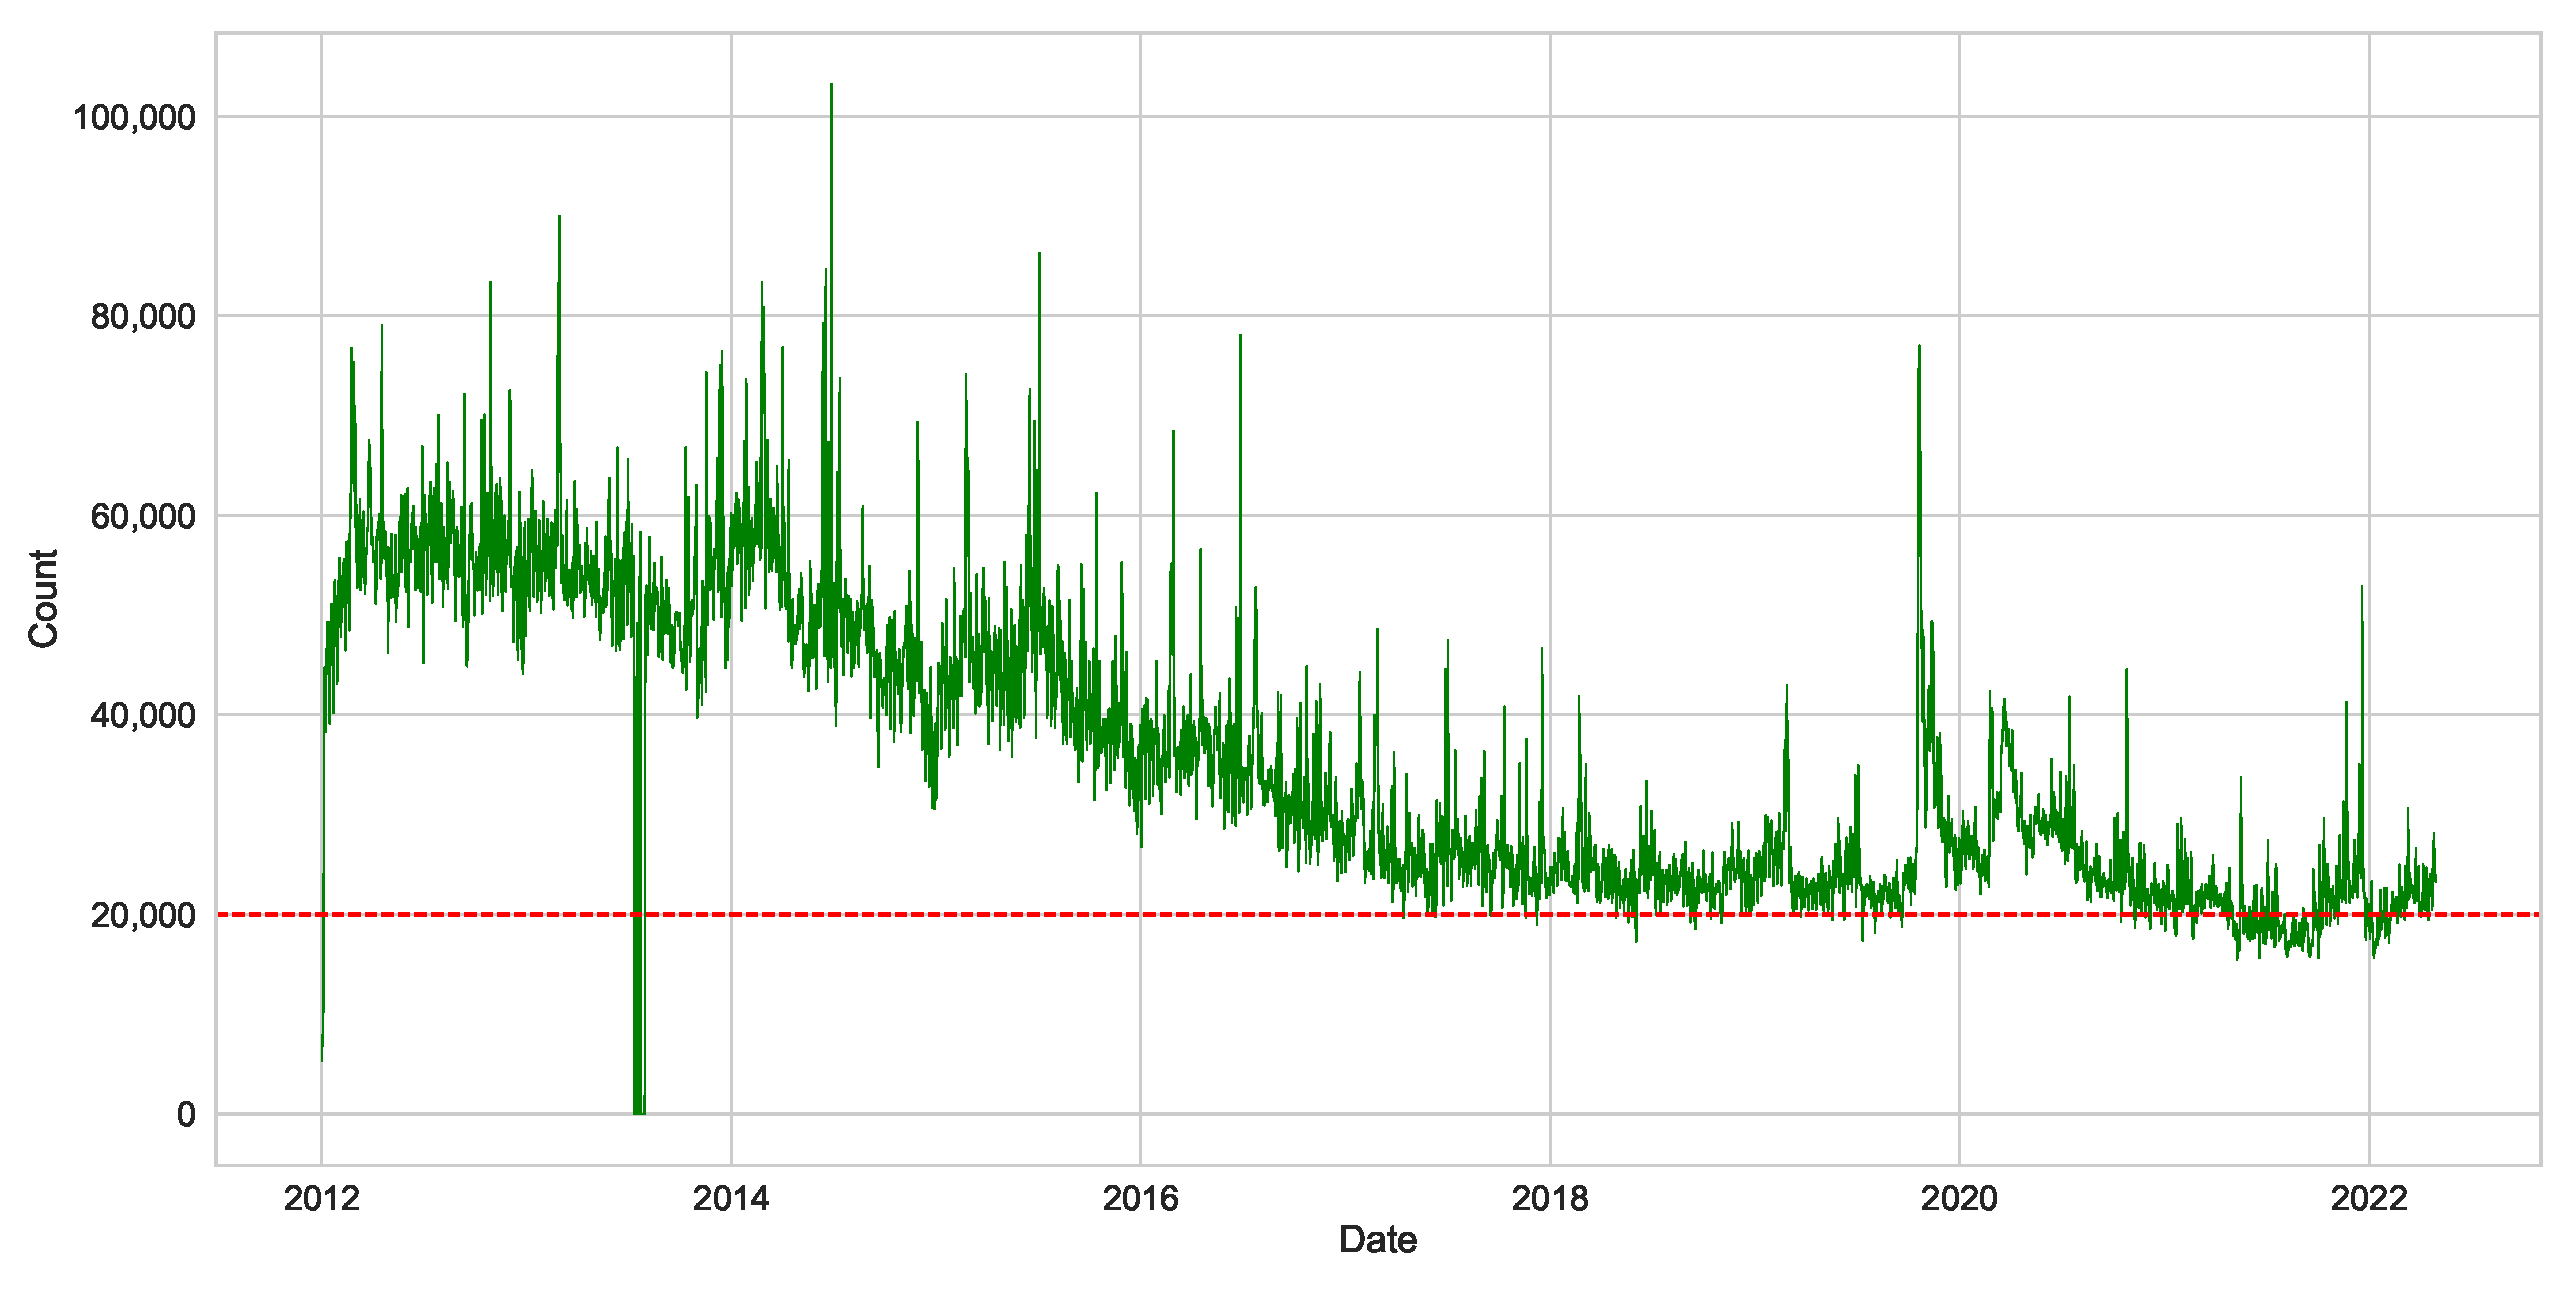
\includegraphics[width = 15cm]{figs/location_tweets_chile_2012_2022}
            \caption{Geotagged Tweets From Chile, 2012--2022}
            \floatfoot{\it Notes: Red dashed line shows lower
            bound of 20,000 tweets. \\ 
            Source: Twitter data downloaded using \texttt{twarc2} API.}
            \label{appfig_loc_twit_chi_12_22}
        \end{figure}
        
        % Figure: Top 20 Author Locations in Corpus
        \begin{figure}[!htb]
            \centering
            \includegraphics[width = 15cm]{figs/top20_auth_locs}
            \caption{Top 20 Author Locations in Corpus After Filtering by Citizens}
            \floatfoot{\it %Notes: Red dashed line shows lower bound of 20,000 tweets. \\ 
            Data Source: Retrieved from Twitter API, spanning the time frame Nov 1\textsuperscript{st}, 2020 -- April 11\textsuperscript{th}, 2022. Corpus includes tweets by Twitter users in Chile or Chilean nationals that mainly pertain to immigration.}
            \label{appfig_top20_auth_locs}
        \end{figure}
        
        \begin{figure}%[H]
             \centering
             \includegraphics[height=.85\textheight]{figs/dash_screen}
             \caption{Screenshot of First Prototype of Interactive Dashboard}
             \label{fig_dash_screen}
             \floatfoot{\it 
                Notes:  Dashboard coded using the Python packages \texttt{Plotly} and \texttt{Dash} and using the corpus from Step 5 as input. Textual preprocessing steps in outputs include lowercase enforcement and converting Spanish special characters (e.g. á, ñ, etc.) into corresponding non-accentuated ones.
                \\ 
                %Data Source: Retrieved from Twitter API utilizing the \texttt{twarc2} command line tool, spanning the time frame Nov 1\textsuperscript{st}, 2020 -- April 11\textsuperscript{th}, 2022. Data is cleaned by our proposed methodology, such that the corpus includes tweets with topic-related keywords (semantic link + country contextual) and are tweeted by Twitter users in Chile or Chilean national Twitter users living abroad and contains tweets that mainly regard the topic of immigration.}
                Data Source: Retrieved from Twitter API, spanning the time frame Nov 1\textsuperscript{st}, 2020 -- April 11\textsuperscript{th}, 2022. Corpus includes tweets by Twitter users in Chile or Chilean nationals that mainly pertain to immigration. Corpus cleaned by the steps in our methodology as described in Section \ref{sec_meth_gene} and Appendix \ref{app_sec_meth}.}
        \end{figure}
        
        % Figure: Wordcloud of Author Biographies in Corpus After Filtering by Citizens
        \begin{figure}[!htb]
            \centering
            \includegraphics[width = 15cm]{figs/auth_desc_cloud}
            \caption{Wordcloud of Author Biographies in Corpus After Filtering by Citizens}
            \floatfoot{\it %Notes: Red dashed line shows lower bound of 20,000 tweets. \\ 
            Data Source: Retrieved from Twitter API, spanning the time frame Nov 1\textsuperscript{st}, 2020 -- April 11\textsuperscript{th}, 2022. Corpus includes tweets by Twitter users in Chile or Chilean nationals that mainly pertain to immigration.}
            \label{appfig_auth_desc_cloud}
        \end{figure}
        
        %\begin{figure}[H]
        %     \centering
        %     \includegraphics[width=.99\linewidth]{figs/Common_Hashtags.eps}
        %     \caption{Most Popular Hashtags, Total Corpus}
        %     \label{popular_hashtags}
        %     \floatfoot{\it 
        %            Notes: Textual preprocessing steps include lowercase enforcement and converting Spanish special characters (e.g. á, ñ, etc.) into corresponding non-accentuated ones.
        %            \\ 
        %            Data Source: \textcolor{red}{$<$mention the corpus where this comes from á la footnote in Table \ref{tab_corpora_characs}$>$}}
        %\end{figure}
        
        %\begin{figure}[H]
        %     \centering
        %     \includegraphics[width=.99\linewidth]{figs/Common_Bigrams.eps}
        %     \caption{Most Popular Bigrams, Total Corpus}
        %     \label{total_bigrams}
        %     \floatfoot{\it 
        %            Notes: Textual preprocessing steps include lowercase enforcement and converting Spanish special characters (e.g. á, ñ, etc.) into corresponding non-accentuated ones.
        %            \\ 
        %            Data Source: \textcolor{red}{$<$mention the corpus where this comes from á la footnote in Table \ref{tab_corpora_characs}$>$}}
        %\end{figure}
        
        %\begin{figure}[H]
        %     \centering
        %     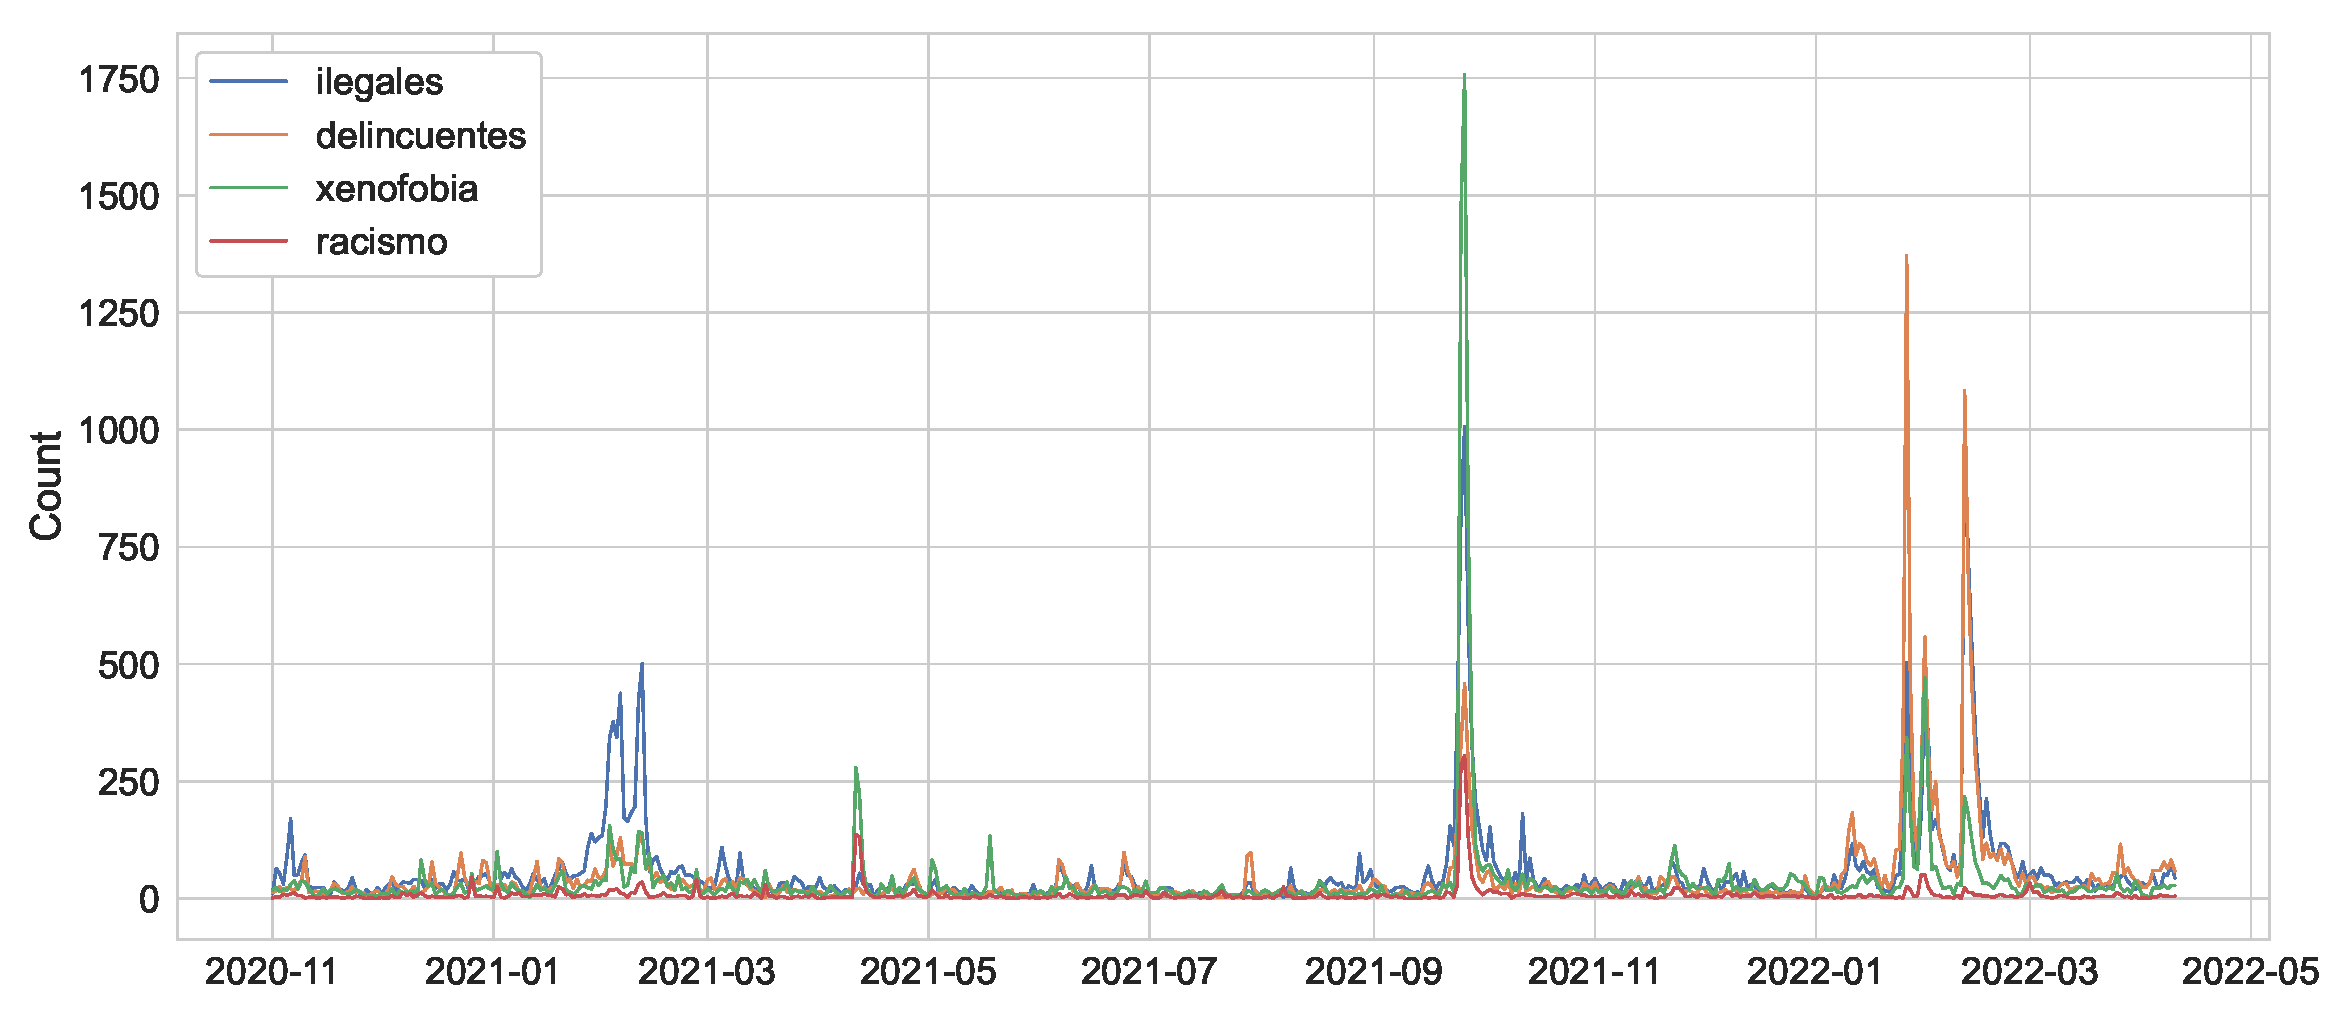
\includegraphics[width=\textwidth]{figs/words_over_time.eps}
        %     \caption{Use of Terms {\it ‘Ilegales’}, {\it ‘Delincuentes’ }, {\it ’Xenofobia’} and {\it ‘Racismo'}; Nov 1, 2020 -- Apr 11, 2022}
        %     \label{appfig_words_over_time}
        %     \floatfoot{\it 
                    %Notes:  \\ 
        %            Data Source: \textcolor{red}{$<$mention the corpus where this comes from á la footnote in Table \ref{tab_corpora_characs}$>$}}
        %\end{figure}
        
        \begin{figure}[H]
             \centering
             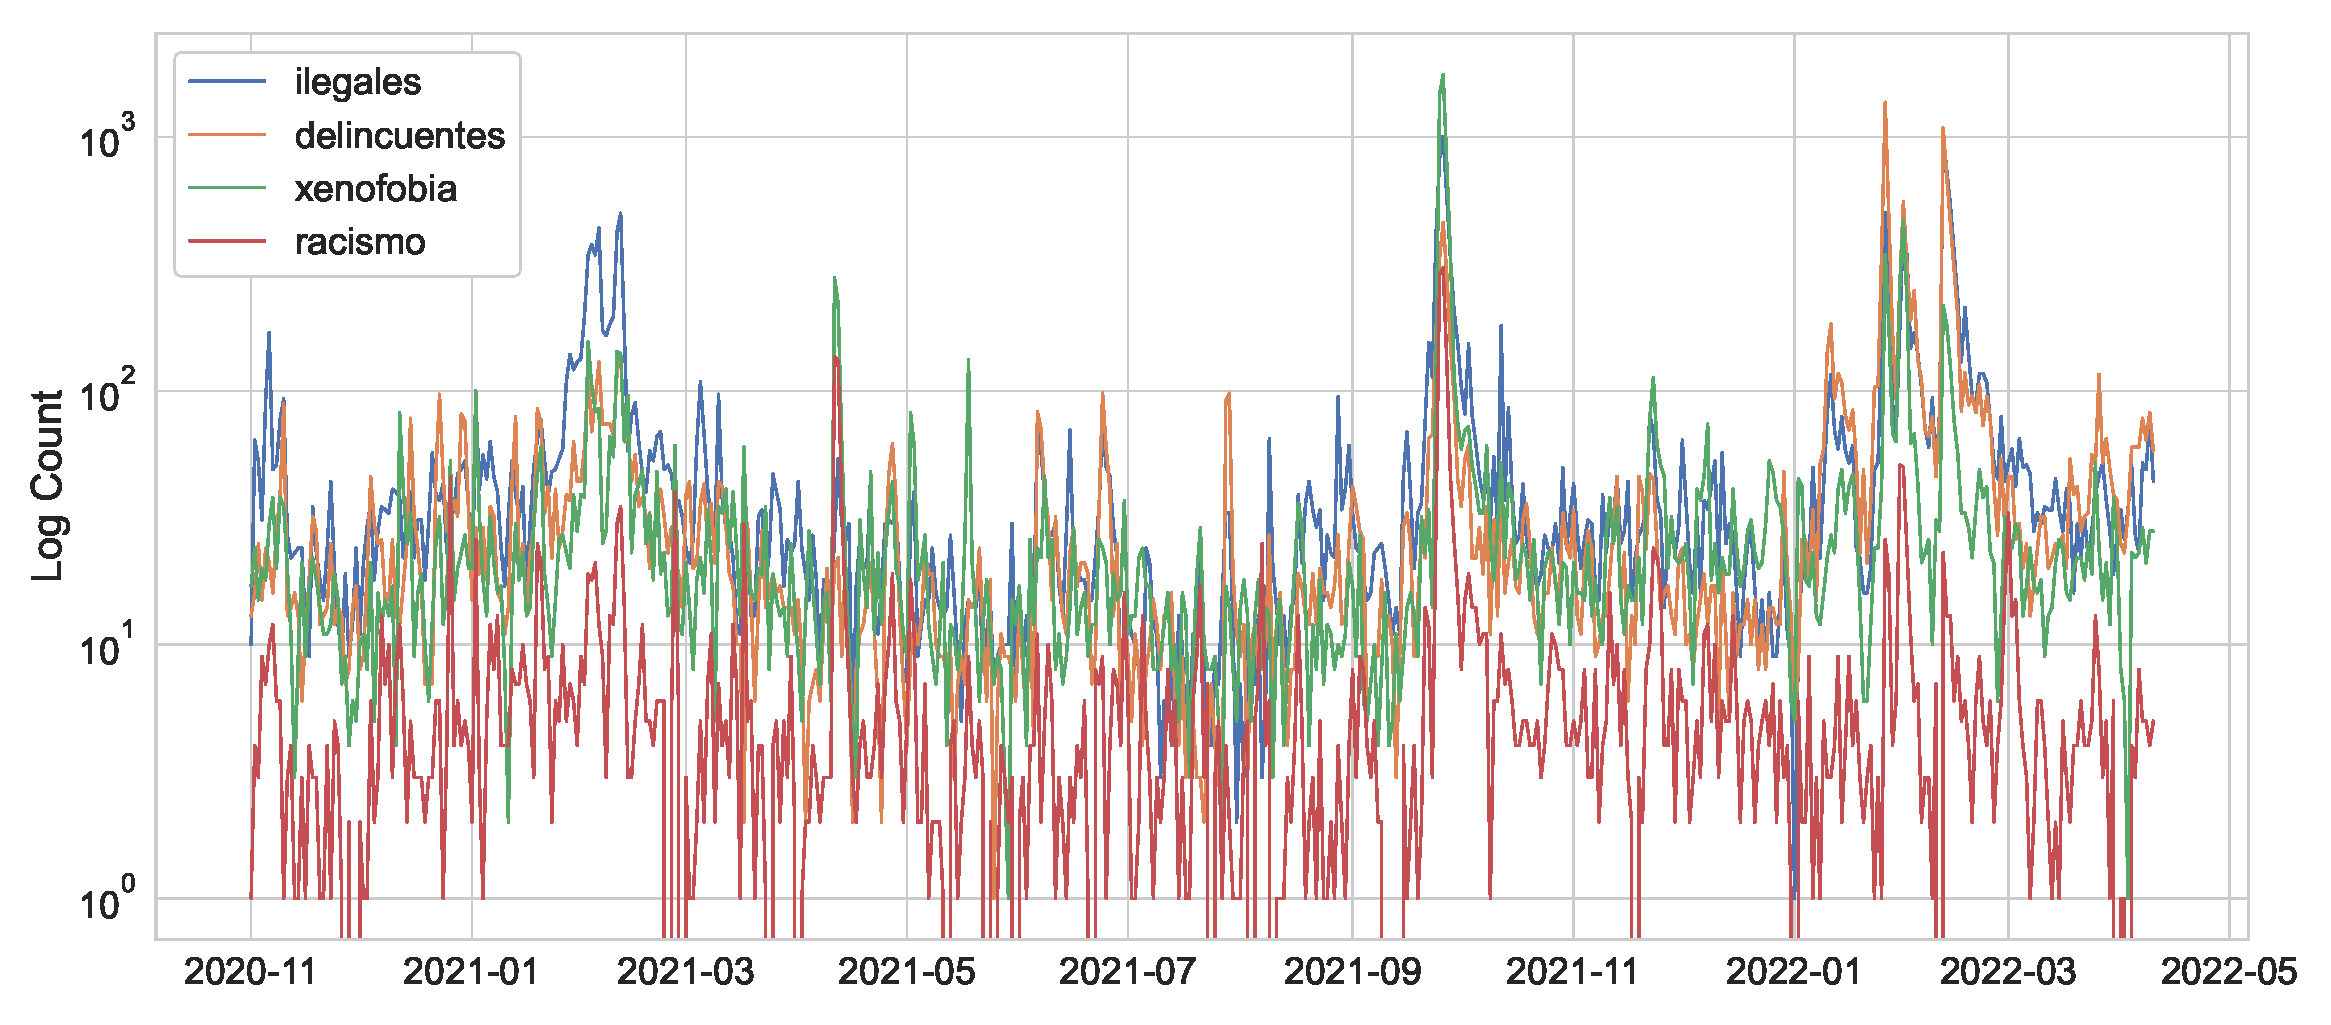
\includegraphics[width=\textwidth]{figs/words_over_time_log.eps}
             \caption{Log Usage of Anti-Immigration and Anti-Xenophobia Terms; Total Corpus}
             \label{fig_words_over_time_log}
             \floatfoot{\it 
                    Notes:  The anti-immigration terms plotted are {\it ‘ilegales’} (Eng: Illegals) and {\it ‘delincuentes’} (Eng: Criminals). The anti-xenophobia terms are {\it ’xenofobia’} (Eng: Xenophobia) and {\it 'racismo'} (Eng: Racism). Textual preprocessing steps include lowercase enforcement and converting Spanish special characters (e.g. á, ñ, etc.) into corresponding non-accentuated ones.
                    \\ 
                    Data Source: Same as Figure \ref{fig_words_over_time}. }
        \end{figure}
        
       \begin{figure}[!htb]
             \centering
             \includegraphics[width=.8\linewidth]{figs/WordCloud_Study.png}
             \caption{Wordcloud for Author Descriptions of Twitter Users That Use Discriminatory Language Towards Immigrants from the SJM Study}
             \label{appfig_cloud_SJM}
             \floatfoot{\it 
                    %Notes:  \\ 
                    Source: \cite{glvez_2020_barmetro}}
        \end{figure}
    
    
    \clearpage
    \begin{figure}[H]
        \caption{Random Author Location and Descriptions after Step 3}
        \label{random_loc_desc}
        
        \centering
            \begin{subfigure}{0.49\textwidth}
                \centering
                \includegraphics[width=.99\linewidth]{figs/chile_author_1.png}
            \end{subfigure}%
        %\hfill
            \begin{subfigure}{0.49\textwidth}
                \centering
                \includegraphics[width=.99\linewidth]{figs/chile_author_2.png}
            \end{subfigure}
        \hfill
            \begin{subfigure}{0.49\textwidth}
                \centering
                \includegraphics[width=.99\linewidth]{figs/chile_author_3.png}
            \end{subfigure}%
        %\hfill
            \begin{subfigure}{0.49\textwidth}
                \centering
                \includegraphics[width=.99\linewidth]{figs/chile_author_4.png}
            \end{subfigure}
        \hfill
            \begin{subfigure}{0.49\textwidth}
                \centering
                \includegraphics[width=.99\linewidth]{figs/chile_author_5.png}
            \end{subfigure}%
        %\hfill
            \begin{subfigure}{0.49\textwidth}
                \centering
                \includegraphics[width=.99\linewidth]{figs/chile_author_6.png}
            \end{subfigure}
    
    \floatfoot{\it 
                %Notes:  Textual preprocessing steps in outputs include lowercase enforcement and converting Spanish special characters (e.g. á, ñ, etc.) into corresponding non-accentuated ones.
                %\vspace{0.5em} \\
                Data Source: Screenshots from Twitter. Retrieved from Twitter API, spanning the time frame Nov 1\textsuperscript{st}, 2020 -- April 11\textsuperscript{th}, 2022. Corpus includes tweets by Twitter users in Chile or Chilean nationals that mainly pertain to immigration. Corpus cleaned by the steps in our methodology as described in Section \ref{sec_meth_gene} and Appendix \ref{app_sec_meth}.}
    \end{figure}
    
        
    
    \clearpage
    \begin{figure}[H]
        \caption{Random Selection of Tweets, Total Corpus}
        \label{random_tweets_tot}
        
        \centering
            \begin{subfigure}{0.49\textwidth}
                \centering
                \includegraphics[width=.99\linewidth]{figs/tweet_general_1.png}
            \end{subfigure}%
        %\hfill
            \begin{subfigure}{0.49\textwidth}
                \centering
                \includegraphics[width=.99\linewidth]{figs/tweet_general_2.png}
            \end{subfigure}
        \hfill
            \begin{subfigure}{0.49\textwidth}
                \centering
                \includegraphics[width=.99\linewidth]{figs/tweet_general_4.png}
            \end{subfigure}%
        %\hfill
            \begin{subfigure}{0.49\textwidth}
                \centering
                \includegraphics[width=.99\linewidth]{figs/tweet_general_5.png}
            \end{subfigure}
        
    \floatfoot{\it 
                %Notes:  Textual preprocessing steps in outputs include lowercase enforcement and converting Spanish special characters (e.g. á, ñ, etc.) into corresponding non-accentuated ones.
                %\vspace{0.5em} \\
                Data Source: Screenshots from Twitter. Corpus resulting after Step 3 in application of methodology to immigration in Chile as described in Appendix \ref{app_sec_meth}. Corpus spans the time frame Nov 1\textsuperscript{st}, 2020 -- April 11\textsuperscript{th}, 2022 and includes tweets by Twitter users in Chile or Chilean nationals that mainly pertain to immigration.}
    \end{figure}
    
    
    \clearpage
    \begin{figure}[H]
        \caption{Random Selection of Tweets, Left-Leaning Users}
        \label{random_tweets_lef}
        
        \centering
            \begin{subfigure}{0.49\textwidth}
                \centering
                \includegraphics[width=.99\linewidth]{figs/tweet_left_1.png}
            \end{subfigure}%
        %\hfill
            \begin{subfigure}{0.49\textwidth}
                \centering
                \includegraphics[width=.99\linewidth]{figs/tweet_left_2.png}
            \end{subfigure}
        \hfill
            \begin{subfigure}{0.49\textwidth}
                \centering
                \includegraphics[width=.99\linewidth]{figs/tweet_left_3.png}
            \end{subfigure}%
        %\hfill
            \begin{subfigure}{0.49\textwidth}
                \centering
                \includegraphics[width=.99\linewidth]{figs/tweet_left_4.png}
            \end{subfigure}
        
    \floatfoot{\it 
                %Notes:  Textual preprocessing steps in outputs include lowercase enforcement and converting Spanish special characters (e.g. á, ñ, etc.) into corresponding non-accentuated ones.
                %\vspace{0.5em} \\
                Data Source: Screenshots from Twitter. Corpus resulting after Step 3 in application of methodology to immigration in Chile as described in Appendix \ref{app_sec_meth}. Corpus spans the time frame Nov 1\textsuperscript{st}, 2020 -- April 11\textsuperscript{th}, 2022 and includes tweets by Twitter users in Chile or Chilean nationals that mainly pertain to immigration.}
    \end{figure}
    
    \clearpage
    \begin{figure}[H]
        \caption{Random Selection of Tweets, Right-Leaning Users}
        \label{random_tweets_rig}
        
        \centering
            \begin{subfigure}{0.49\textwidth}
                \centering
                \includegraphics[width=.99\linewidth]{figs/tweet_right_1.png}
            \end{subfigure}%
        %\hfill
            \begin{subfigure}{0.49\textwidth}
                \centering
                \includegraphics[width=.99\linewidth]{figs/tweet_right_2.png}
            \end{subfigure}
        \hfill
            \begin{subfigure}{0.49\textwidth}
                \centering
                \includegraphics[width=.99\linewidth]{figs/tweet_right_3.png}
            \end{subfigure}%
        %\hfill
            \begin{subfigure}{0.49\textwidth}
                \centering
                \includegraphics[width=.99\linewidth]{figs/tweet_right_4.png}
            \end{subfigure}
        
    \floatfoot{\it 
                %Notes:  Textual preprocessing steps in outputs include lowercase enforcement and converting Spanish special characters (e.g. á, ñ, etc.) into corresponding non-accentuated ones.
                %\vspace{0.5em} \\
                Data Source: Screenshots from Twitter. Corpus resulting after Step 3 in application of methodology to immigration in Chile as described in Appendix \ref{app_sec_meth}. Corpus spans the time frame Nov 1\textsuperscript{st}, 2020 -- April 11\textsuperscript{th}, 2022 and includes tweets by Twitter users in Chile or Chilean nationals that mainly pertain to immigration.}
    \end{figure}
    
    
        
        % \newpage
        % \subsubsection{Random Author Location and Descriptions after Step 3}\label{random_loc_desc}
        %     \epigraph{''ID: $<$censored$>$ \\
        %     Location: Chile \\
        %     Description: Diseñador Industrial \| Artista 3D\&CGI \| Fotógrafo Aficionado. :camera:  \|\|  Industrial Designer \| 3D&3D\&CGI Artist \| Amateur Photographer. :camera:''}{}
            
        %     \epigraph{''ID: $<$censored$>$ \\
        %     Location: Santiago,Chile  \\
        %     Description: ¡Súmate al camino de la ERRADICACIÓN de la situación de calle y la recuperación de DERECHOS! Teléfono: $<$censored$>$. E-mail: $<$censored$>$''}{}
            
        %     \epigraph{''ID: $<$censored$>$ \\
        %     Location: nan  \\
        %     Description: El innombrable mechero, oportunista y basura política. Nunca será mi presidente. Mi Chile lindo! nunca quiero perderte''}{}
            
        %     \epigraph{''ID: $<$censored$>$ \\
        %     Location: Chile  \\
        %     Description: Curacautin, Araucania, Chile''}{}
            
        %     \epigraph{''ID: $<$censored$>$ \\
        %     Location: Aculeo. Santiago de Chile.
        %     Description: Ingeniero Civil Matemático. Doctor en Ingeniería de Minas. Presidente Federación de Biathlón de Chile''}{}
            
        %     \epigraph{''ID: $<$censored$>$ \\
        %     Location: Chile   \\
        %     Description: "La educación te hace libre, la ignorancia esclavo."''}{}
            
        %     \epigraph{''ID: $<$censored$>$ \\
        %     Location: Santiago de Chile   \\
        %     Description: Ciudadana del mundo.:globe\_showing\_Asia-Australia::milky\_way: Eres lo que haces, no lo que dices que vas hacer .
        %     ''}{}
            
        %     \epigraph{''ID: $<$censored$>$ \\
        %     Location: Valparaíso, Chile.  \\
        %     Description: Porteño y Periodista :railway\_car::movie\_camera:''}{}
            
        % \newpage
        %     \epigraph{''ID: $<$censored$>$ \\
        %     Location: Santiago, Chile  \\
        %     Description: No mas \#SERVICIOJESUITAMIGRANTE en Chile \#NomasONU . Singapurista a la chilena, chilenials chilenialista. SÍGUEME Y TE SIGO .''}{}
            
        %     %\epigraph{''ID: $<$censored$>$ \\
        %     %Location: nan
        %     %Description: O la tiranía marxista o la libertad.:Statue_of_Liberty: Republicana:Chile:Anticomunista Resistencia Patriota :Chile: Rechazo:Chile:22\%/44\% Kast por siempre:victory_hand::growing_heart::Chile:''}{}
        